\subsection{Benchmarks}
\makesubcontentsslidessec

\begin{frame}
  \begin{block}{Default Choices Throughout}
    \begin{itemize}[<+-|alert@+>]
      \item Only free software used (no MKL, ACML, etc.)
      \item Generate random matrix
        \begin{itemize}
        \item Global Columns: 500, 1000, and 2000
        \item Global Rows: vary with core count (local matrix fixed at
          $43.4 MiB$)
        \end{itemize}
      \item 1 core = 1 MPI process
      \item Measure wall clock time
      \item ``weak scaling'' = global problem grows with core count
    \end{itemize}
    \vspace{.8cm}
    \centering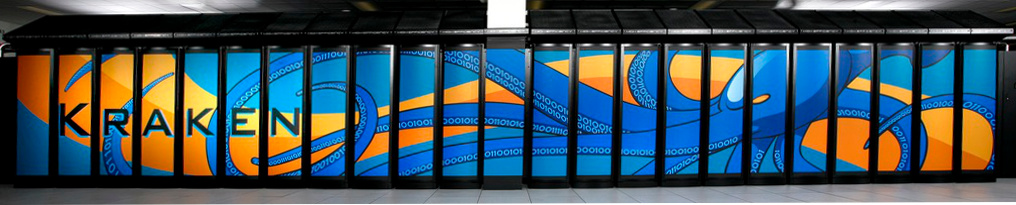
\includegraphics{../common/pics/krakenWide}
  \end{block}
\end{frame}

\begin{frame}[fragile]
  \begin{block}{Covariance Benchmark (pbdDMAT)}
    \vspace{-3ex}\scriptsize
    \begin{lstlisting}
x <- ddmatrix("rnorm", nrow=n, ncol=p, mean=mean, sd=sd)
cov.x <- cov(x)
    \end{lstlisting}
    \vspace{-4ex}
    \begin{center}
      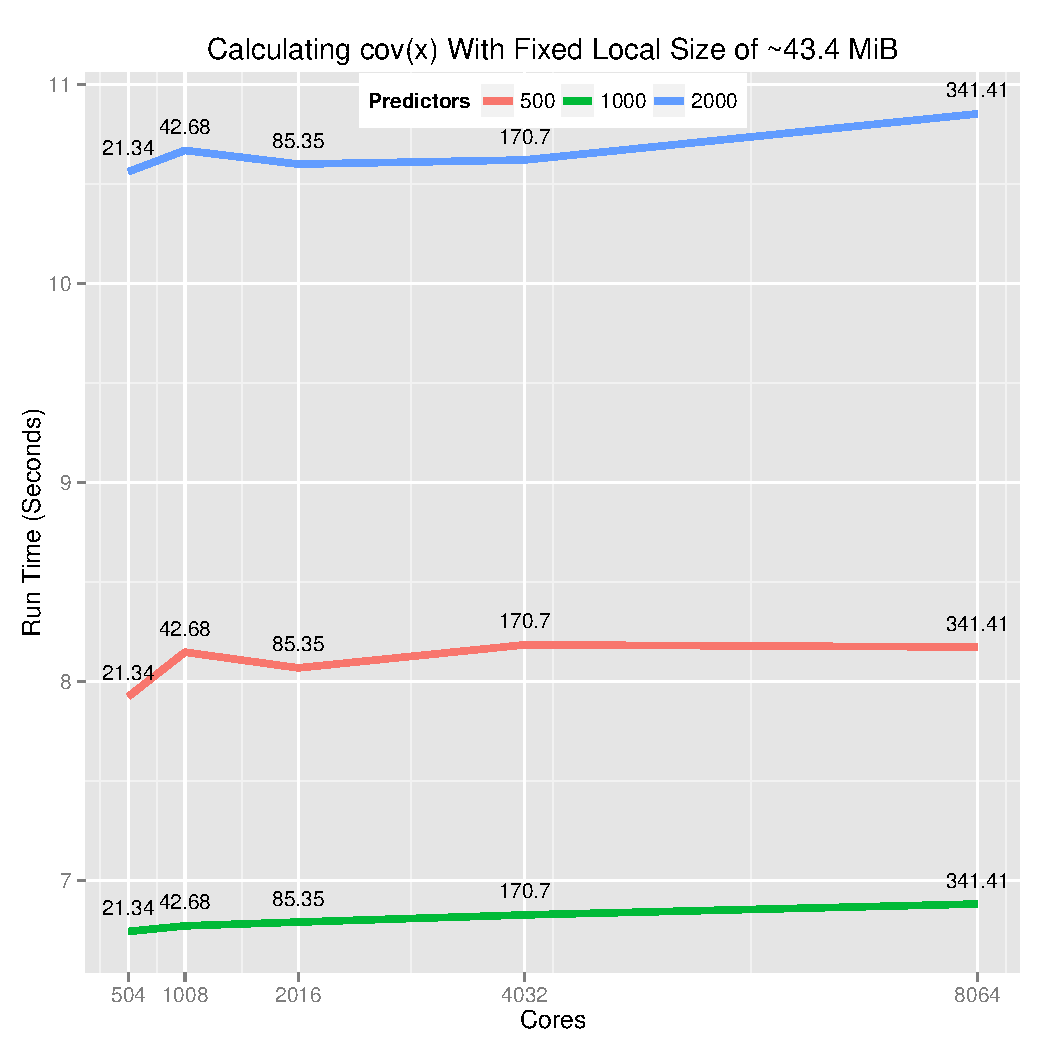
\includegraphics[trim=3mm 1mm 2mm 11.5mm,clip,height=.78\textheight]{../common/pics/cov}
    \end{center}
  \end{block}
\end{frame}

\begin{frame}[fragile]
  \begin{block}{Linear Regression Benchmark (pbdDMAT)}
    \vspace{-3.5ex}\scriptsize
    \begin{lstlisting}
beta.true <- ddmatrix("runif", nrow=p, ncol=1)
y <- x %*% beta.true
beta.est <- lm.fit(x, y)$coefficients
    \end{lstlisting} %$
    \vspace{-3ex}
    \begin{center}
      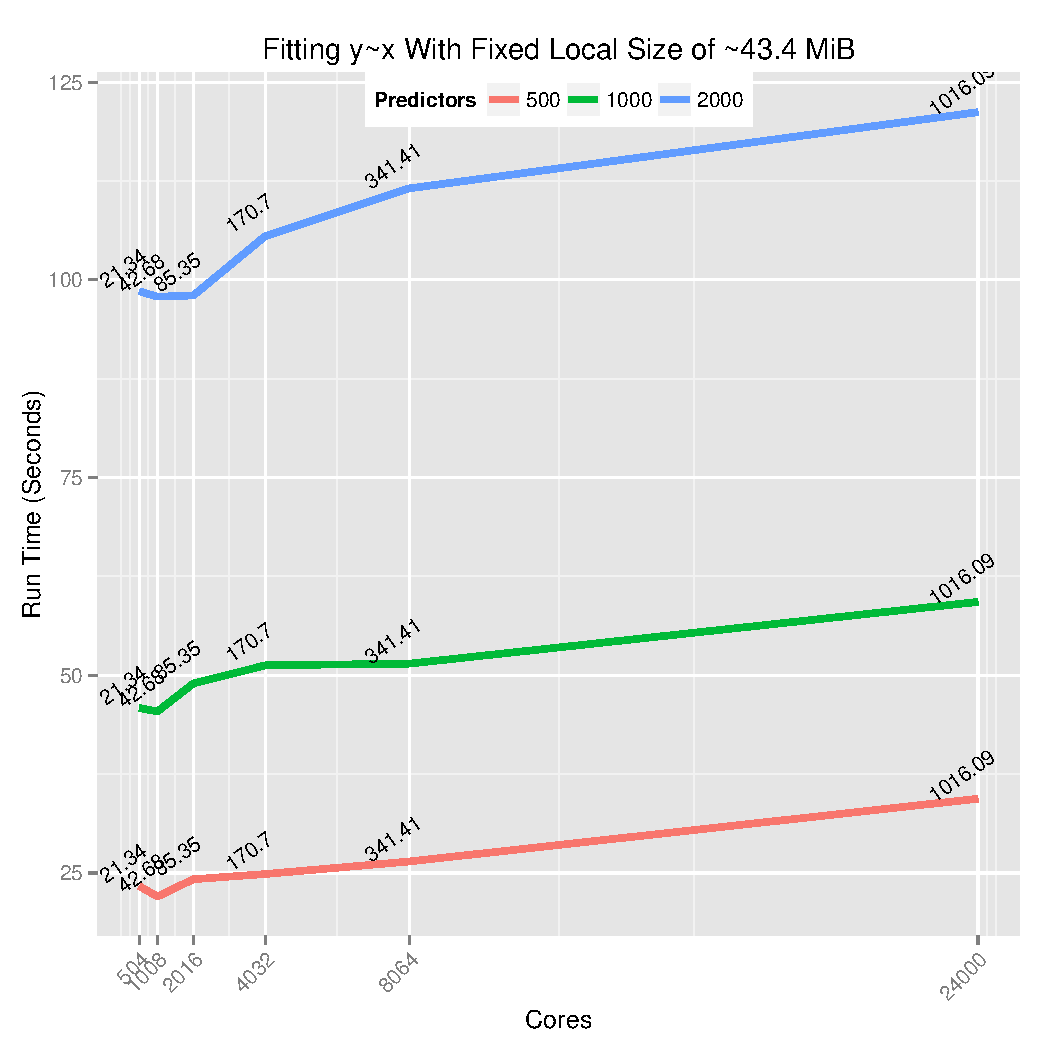
\includegraphics[trim=3mm 1mm 2mm
      11.2mm,clip,height=.77\textheight]{../common/pics/benchmarks/lmfit2}
    \end{center}
  \end{block}
\end{frame}

\begin{frame}
  \begin{block}{\code{Data Generation (pbdDMAT)}}
  \begin{center}
    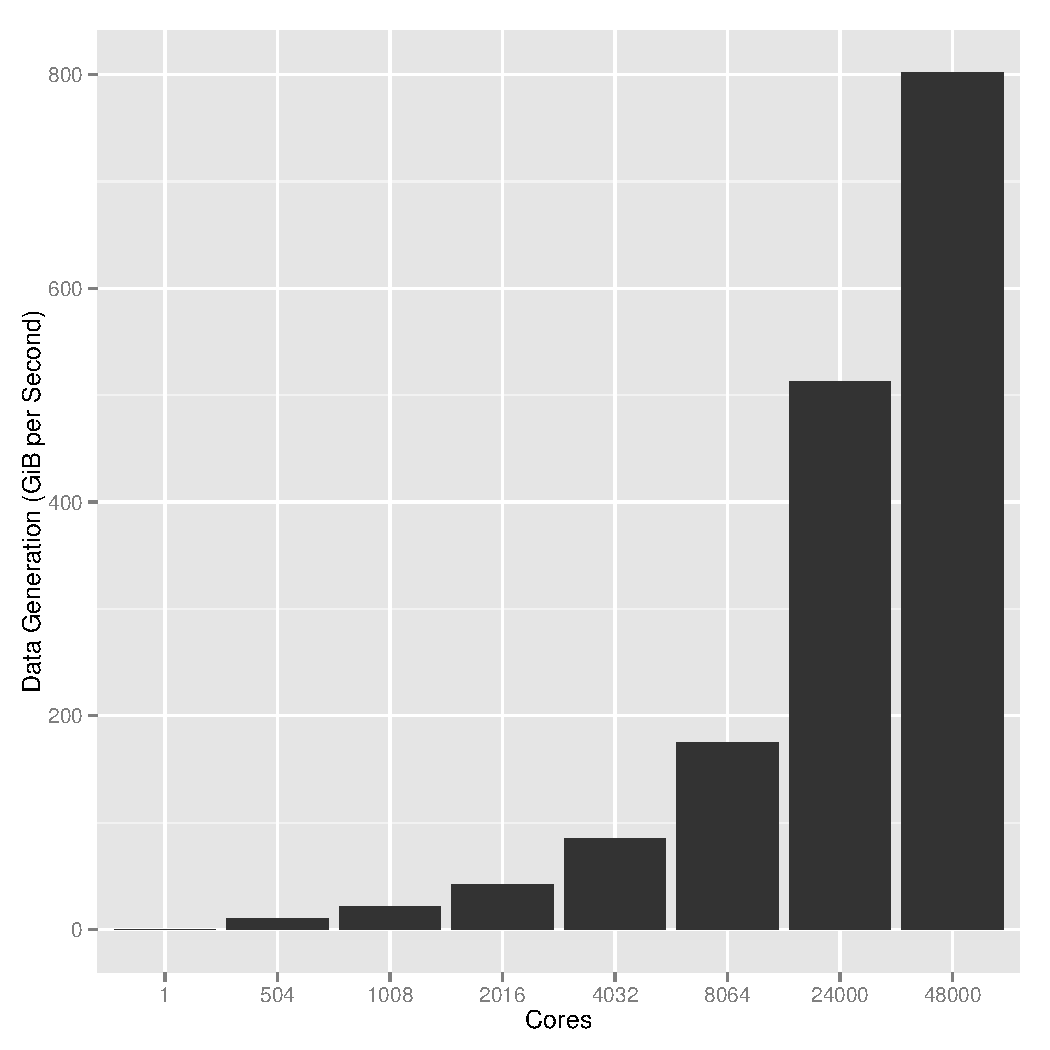
\includegraphics[height=.88\textheight]{../common/pics/benchmarks/datagen24k}
  \end{center}
  \end{block}
\end{frame}

\begin{frame}
  \begin{block}{Matrix Exponentiation (pbdDMAT)}
    \begin{minipage}{5cm}
      \begin{itemize}\tiny
      \item Fitting biogeography models requires many matrix exponentiations
      \item Benchmark: Matrix exponential of 5000$\times$5000 matrix.
      \item R 3.1.0, Matrix 1.1-2, rexpokit 0.25, pbdDMAT 0.3-0
      \item Libs: Cray LibSci, NETLIB ScaLAPACK, Compilers: gnu 4.8.2
      \item Configuration: 1 thread == 1 MPI rank == 1 physical core
      \end{itemize}
      \vspace{-4ex}
      \begin{center}
        \includegraphics[trim=4cm 2cm 3.5cm 2.2cm,clip=true,height=4cm]{pics/Biogeography}
      \end{center}
    \end{minipage}
    \begin{minipage}{6.9cm}
      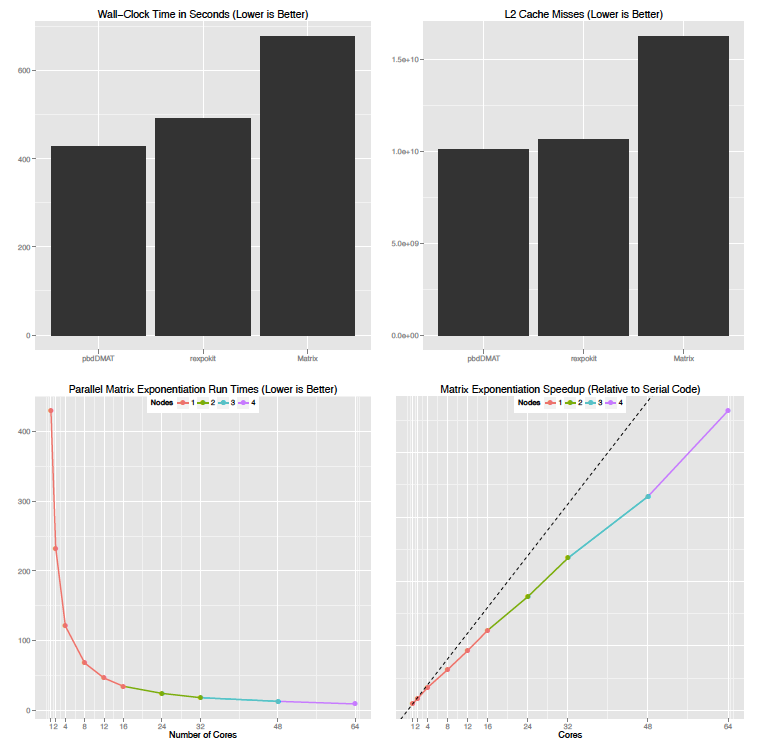
\includegraphics[trim=1mm 1mm 1mm 1mm,clip=true,height=7cm]{pics/MatExp}
    \end{minipage}
  \end{block}
  \begin{raggedright}\tiny
    Schmidt and Matzke (2014) Distributed matrix exponentiation, The R
    User Conference (UseR! 2014), \\[-2ex] Los Angeles, CA, August 2014 .
  \end{raggedright}
\end{frame}

% \begin{frame}
%   \begin{block}{\code{prcomp() Strong Scaling (pbdDMAT)}}
%   \begin{center}
%     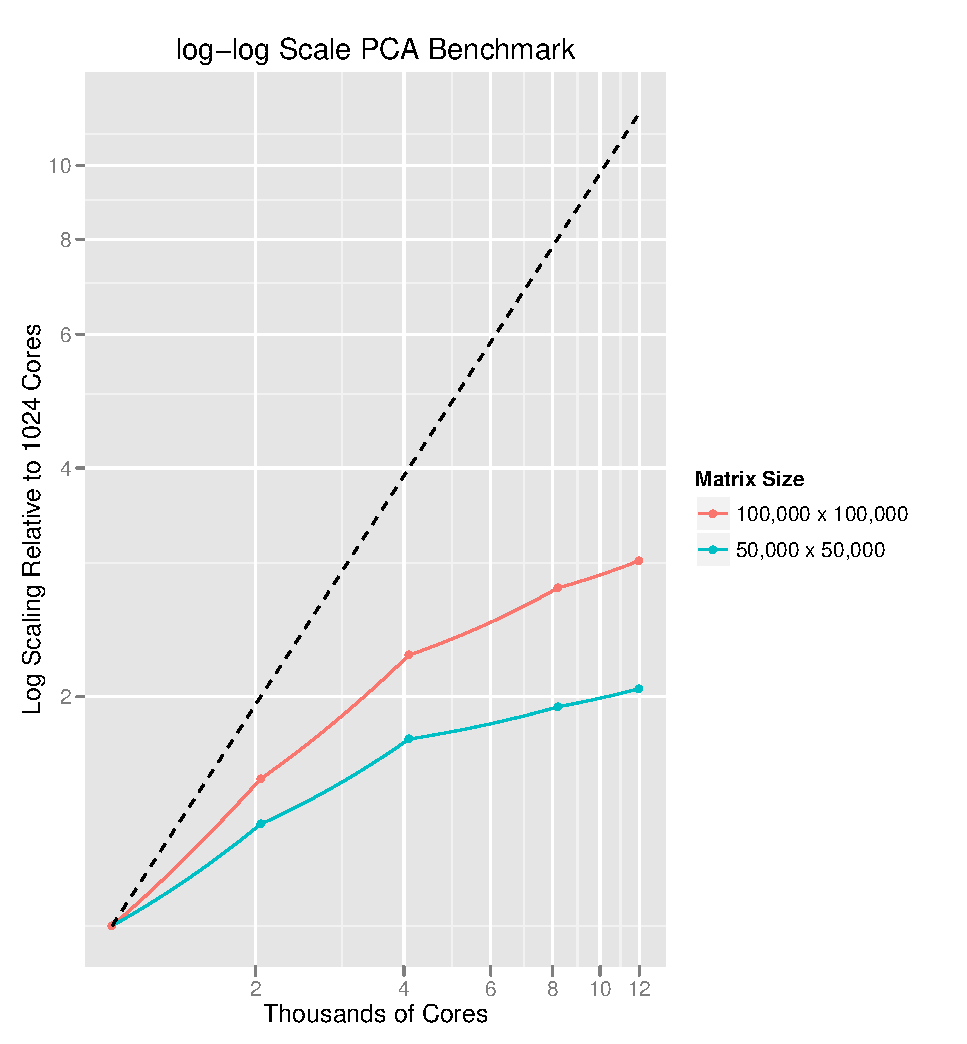
\includegraphics[height=.88\textheight]{../common/pics/benchmarks/pca_scaling}
%   \end{center}
%   \end{block}
% \end{frame}